\section{ Label Based Authorization Model (LaBAC)}
\label{sec:labac}

In \textit{LaBAC}, we assign each object a label named \emph{object-label} and each user another label named \emph{user-label}. In general, a label (both user-label and object-label) is a set valued assigned attribute and its values form a partial order. In LaBAC, we specify policies  in the form of  (\emph{user-label} values, \emph{action},  \emph{object-label} values)   which means that objects labeled with any of \textit{object-label} values are allowed to be accessed by the users labeled with any of  \textit{user-label }values for the specific \textit{action}.  The formal definition of the model is shown in Table \ref{table:labac-formal-model}.


\begin{figure*}
\centering
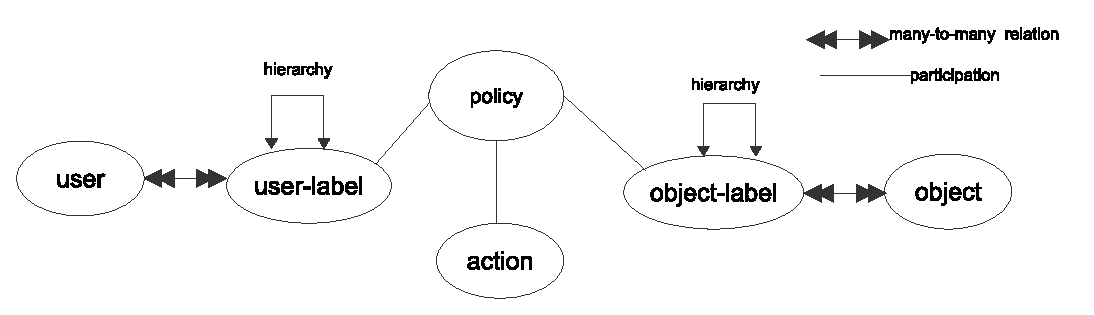
\includegraphics[width=1\textwidth]{labac-model.eps}
\caption{Label Based Access Control Model.}
\label{fig:labac-model}
\end{figure*}

%===================Policy Configuration starts ==================%
\begin{table*}[t] \footnotesize
\centering
\caption{LaBAC - Formal Definition}
\label{table:labac-formal-model}
\begin{tabular}{p{\textwidth}}

\hline
\noindent \textbf{ Primitives Sets:} \\
$U, O, A$: finite set of existing users, objects and actions respectively. \\
$UL, OL$: finite set of existing user-label values  and object-label values respectively. \\
\noindent \textbf{Relations} \\
$ULH \subseteq UL \times UL$  is a partial order on user-label values called inheritance relation written as $\succeq_{ul}$, where $ul_i \succeq_{ul} ul_j$ if all users of $ul_i$ are also users of $ul_j$. Formally $ul_i \succeq_{ul} ul_j$ if $users(ul_i) \subseteq users(ul_j)$. \\

$OLH \subseteq OL \times OL$  is a partial order on object-label values called inheritance relation on objects written as $\succeq_{ol}$, where $ol_i \succeq_{ol} ol_j$ if all objects of $ol_j$ are also objects of $ol_i$. Formally $ol_i \succeq_{ol} ol_j$ if $objectss(ol_j) \subseteq objects(ol_i)$. \\\\


$Policy \subseteq UL \times A \times OL$ is a mapping of user-labels, action of object-labels.\\

$UUA \subseteq U \times UL$ is the user to user-label value assignment relation.  \\ 
$OOA \subseteq O \times OL$ is the object to object-label value assignment relation. \\ 
$UP \subseteq U \times A \times O$ is a computed relation specifying  permissible user permission set.  \\ 
\noindent $UP= \{  (u,o,a) | u \in users(ul_i), o \in objects(ol_j)    \exists ul_i [ul_i \in UL ] (ul_i \succeq_{ul} ul) \exists ol_i [ol_i \in OL] (ol \succeq_{ol} ol_j) (ul,a,ol) \in Policy     \} $ \\
\noindent \textbf{Mapping functions:}\\
object\_labels: $(o:O) \to \{ ol \in OL | (o,ol) \in OOA\}$ \\
user\_labels: $(u:U) \to \{ ul \in UL | (u,ul) \in UUA\}$ \\
objects:$(ol:OL) \to \{o \in O | (o,ol) \in OOA\} $\\
users:$(ul:UL) \to \{u \in U | (u,ul) \in UUA\} $\\

\hline
\end{tabular}
\end{table*}

%===================Configuration end ==================%

%\subsection{LaBAC vs Lattice Based Access Control(LBAC)}
%Due to similarity of LaBAC with LBAC \cite{lbac}, we distinguish LaBAC and LBAC.
%
%\begin{itemize}
%	\item \emph{One Security Lattice vs. Two Different Lattices:} Both LBAC and LaBAC has one attribute on users which is user-label in LaBAC and clearance in LBAC, one attribute on object which is object-label on LaBAC and classification in LBAC. But in LBAC, values of user clearance and object classification come from same the security lattice or partially ordered values. But in case of LaBAC, we have separate lattices (or partially ordered values) for user-label and object-label. Distinguishing values for user-label and object-label is important because in practice often these values may come from different sources. 
%	%For example, user clearance values may come from the Human Resource team whereas object classification values may be set by team working working on the objects, or dictated by the organization policy. 
%	
%	\item \emph{Fixed Authorization Rules vs. Flexible Rules:} Information flow or authorization actions(e.g. read, write,etc) in LBAC is dominated by two simple rule namely \emph{Read down} or \emph{Write up} \cite{lbac}. In LaBAC, authorization action is controlled by flexible authorization policies. Flexible authorization policies are important because: 1.  in practice, we often need less restricted policies than Mandatory Access Control and 2.  in order to support two different set of partially ordered values, we need a separate configuration point.
%	
%	\item \emph{User Subject Distinction:} In LBAC, the distinction between user and subjects is recognized. For example, a secret user can perform his actions either by means of a secret subject or a unclassified subject. But for simplicity user-subject distinction is not available in LaBAC.
%\end{itemize}
